\documentclass[11pt,a4paper]{article}

% ==============================================================================
% 1. Mathematical Foundations & Microtypography
% ==============================================================================
\usepackage[utf8]{inputenc}
\usepackage[T1]{fontenc}
\usepackage{amsmath,amssymb,amsfonts,amsthm,bm,mathtools}
\usepackage{microtype}

% ==============================================================================
% 2. Page Geometry & Header/Footer Architecture
% ==============================================================================
\usepackage[margin=1in,headheight=14pt,headsep=15pt,footskip=25pt]{geometry}
\usepackage{fancyhdr}
\pagestyle{fancy}
\fancyhf{}
\lhead{\small\textbf{Lin Anfan (Norman)} \quad SID: \texttt{20861656}}
\rhead{\small\textbf{HKUST COMP 4421 (Fall 2026) --- Assignment 1}}
\cfoot{\small Page \thepage}
\renewcommand{\headrulewidth}{0.5pt}
\renewcommand{\footrulewidth}{0.3pt}

% ==============================================================================
% 3. Tables & Floating Environments
% ==============================================================================
\usepackage{graphicx}
\graphicspath{{../outputs/}{outputs/}}
\usepackage{subcaption}
\usepackage{booktabs,tabularx,multirow,array}
\usepackage{caption}
\captionsetup{font=small,labelfont=bf,labelsep=period}
\captionsetup[subfigure]{font=footnotesize,labelfont=bf,labelsep=period}

% ==============================================================================
% 4. Code Listings (MATLAB Syntax Highlighting)
% ==============================================================================
\usepackage{xcolor}
\usepackage{listings}

\definecolor{matlabgreen}{RGB}{28, 134, 38}
\definecolor{matlabborder}{RGB}{225, 225, 225}
\definecolor{matlabbg}{RGB}{252, 252, 252}
\definecolor{matlabblue}{RGB}{0, 0, 255}
\definecolor{matlabpurple}{RGB}{160, 32, 240}
\definecolor{matlabgray}{RGB}{110, 110, 110}

\lstdefinestyle{matlabstyle}{
    language=Matlab,
    backgroundcolor=\color{matlabbg},
    basicstyle=\ttfamily\scriptsize,
    keywordstyle=\color{matlabblue}\bfseries,
    commentstyle=\color{matlabgreen}\itshape,
    stringstyle=\color{matlabpurple},
    numberstyle=\tiny\color{matlabgray},
    numbers=left,
    stepnumber=1,
    numbersep=6pt,
    frame=single,
    rulecolor=\color{matlabborder},
    tabsize=4,
    breaklines=true,
    breakatwhitespace=false,
    showstringspaces=false,
    captionpos=b,
    keepspaces=true
}
\lstset{style=matlabstyle}

% ==============================================================================
% 5. Hyperlinks & PDF Metadata
% ==============================================================================
\usepackage{hyperref}
\hypersetup{
    colorlinks=true,
    linkcolor=blue!70!black,
    citecolor=blue!70!black,
    urlcolor=blue!70!black,
    pdfauthor={Lin Anfan (Norman)},
    pdftitle={COMP4421 Assignment 1 Written Answers}
}

% ==============================================================================
% Document Title Configuration
% ==============================================================================
\title{\vspace{-1.2cm}\LARGE\textbf{HKUST COMP 4421: Digital Image Processing}\\[0.3em]
\Large\textbf{Assignment 1 Formal Solutions and Engineering Report}}
\author{\textbf{Lin Anfan (Norman)} \quad SID: \texttt{20861656} \quad Dept. of Mathematics (CS Track)}
\date{Fall Semester 2026-27}

\begin{document}
\maketitle
\thispagestyle{fancy}

\hrule
\vspace{0.6em}
\noindent\textbf{Course Architecture \& Official AI Policy Compliance:}\\
In strict accordance with the HKUST COMP 4421 syllabus regulations (\textit{"Students are free to use generative AI on their works, and should acknowledge it when used"}), generative AI models were employed in an auxiliary, consultative capacity for algebraic cross-verification, script boundary validation, and typesetting optimization. All mathematical derivations, algorithmic implementations, experimental code, and written responses were independently executed, audited, and mathematically verified by the author. A full statement is documented in Appendix~\ref{sec:ai_acknowledgment}.
\vspace{0.5em}
\hrule
\vspace{1.0em}

% ==============================================================================
% SECTION 1: PROBLEM 1
% ==============================================================================
\section{Problem 1: Image Arithmetic and Histograms (10 pts)}

\subsection{Mathematical Framework}
Let $\Omega = \{ (x, y) \in \mathbb{Z}^2 \mid 0 \le x < M, \, 0 \le y < N \}$ denote the discrete spatial lattice of dimensions $M = 40$ and $N = 50$, with total spatial cardinality $|\Omega| = 2000$. Pixel intensities are quantized on the 5-bit discrete integer ring $\mathbb{Z}_{32} = \{0, 1, \dots, 31\}$. Image $A$ is formalized as a constant homogeneous field $A(x, y) \equiv 6$, and Image $B$ is characterized by its empirical histogram counts $n_B(r) = \#\{(x, y) \in \Omega \mid B(x, y) = r\}$.

\subsection{(a) Saturated Addition Analysis (5 pts)}
The composite image $C$ is constructed via the pointwise non-linear saturation addition operator:
\begin{equation}
C(x, y) = \min\left( A(x, y) + B(x, y), \; 31 \right) = \min\left( B(x, y) + 6, \; 31 \right).
\end{equation}
Let $\mathcal{T}: \mathbb{Z}_{32} \to \mathbb{Z}_{32}$ be the forward intensity mapping $\mathcal{T}(r) = \min(r + 6, 31)$. The resulting histogram $n_C(c)$ represents the push-forward measure under $\mathcal{T}$:
\begin{equation}
n_C(c) = \sum_{r \in \mathbb{Z}_{32} : \mathcal{T}(r) = c} n_B(r).
\end{equation}
For input bins $r \in \{0, 2, 5, 10, 15, 20\}$, the mapping $\mathcal{T}$ is strictly bijective into $C \in \{6, 8, 11, 16, 21, 26\}$:
\begin{align*}
r &= 0 \implies C = \min(6, 31) = 6 \quad (n_C = 100), & r &= 10 \implies C = \min(16, 31) = 16 \quad (n_C = 300), \\
r &= 2 \implies C = \min(8, 31) = 8 \quad (n_C = 150), & r &= 15 \implies C = \min(21, 31) = 21 \quad (n_C = 300), \\
r &= 5 \implies C = \min(11, 31) = 11 \quad (n_C = 250), & r &= 20 \implies C = \min(26, 31) = 26 \quad (n_C = 300).
\end{align*}
For all intensity levels satisfying $r + 6 \ge 31$ (the boundary saturation regime $r \in \{25, 27, 29, 31\}$), the transformation collapses onto the upper saturation boundary $C = 31$:
\begin{align*}
r = 25 &\implies \min(31, 31) = 31 \quad (n_B = 250), & r = 29 &\implies \min(35, 31) = 31 \quad (n_B = 100), \\
r = 27 &\implies \min(33, 31) = 31 \quad (n_B = 150), & r = 31 &\implies \min(37, 31) = 31 \quad (n_B = 100).
\end{align*}
Summing the collapsed boundary pre-images yields the saturated boundary count:
\begin{equation}
n_C(31) = n_B(25) + n_B(27) + n_B(29) + n_B(31) = 250 + 150 + 100 + 100 = 600.
\end{equation}
The mapping progression and the resulting non-zero histogram bins of $C$ are summarized in Tables~\ref{tab:p1_mapping} and~\ref{tab:p1_hist_C}.

\begin{table}[htbp]
\centering
\small
\begin{minipage}[t]{0.48\textwidth}
\centering
\caption{Pointwise Saturated Addition Mapping.}
\label{tab:p1_mapping}
\begin{tabular}{cccc}
\toprule
\textbf{$r$} & \textbf{$n_B(r)$} & \textbf{$r + 6$} & \textbf{$C = \min(r+6, 31)$} \\
\midrule
0  & 100 & 6  & \textbf{6}  \\
2  & 150 & 8  & \textbf{8}  \\
5  & 250 & 11 & \textbf{11} \\
10 & 300 & 16 & \textbf{16} \\
15 & 300 & 21 & \textbf{21} \\
20 & 300 & 26 & \textbf{26} \\
25 & 250 & 31 & \textbf{31} \\
27 & 150 & 33 & \textbf{31} \\
29 & 100 & 35 & \textbf{31} \\
31 & 100 & 37 & \textbf{31} \\
\bottomrule
\end{tabular}
\end{minipage}\hfill
\begin{minipage}[t]{0.48\textwidth}
\centering
\caption{Non-Zero Histogram Bins of Image $C$.}
\label{tab:p1_hist_C}
\begin{tabular}{ccc}
\toprule
\textbf{Level ($c$)} & \textbf{Count ($n_C$)} & \textbf{Probability ($p_C = n_C/|\Omega|$)} \\
\midrule
6  & 100 & $100 / 2000 = 0.050$ \\
8  & 150 & $150 / 2000 = 0.075$ \\
11 & 250 & $250 / 2000 = 0.125$ \\
16 & 300 & $300 / 2000 = 0.150$ \\
21 & 300 & $300 / 2000 = 0.150$ \\
26 & 300 & $300 / 2000 = 0.150$ \\
31 & 600 & $600 / 2000 = 0.300$ \\
\midrule
\textbf{Total} & \textbf{2000} & \textbf{1.000} \\
\bottomrule
\end{tabular}
\end{minipage}
\end{table}

\noindent\textbf{Measure Conservation Verification:}
$\sum_{c} n_C(c) = 100 + 150 + 250 + 300 + 300 + 300 + 600 = 2000 = |\Omega|$. \quad (\textit{Q.E.D.})

\subsection{(b) Difference Imaging and Dynamic Classification (5 pts)}
Let $I_{\text{before}}, I_{\text{after}}: \Omega \to \mathbb{Z}_{32}$. The signed difference image is $D(x, y) = I_{\text{after}}(x, y) - I_{\text{before}}(x, y) \in \{-31, \dots, 31\}$.
\begin{itemize}
    \item \textbf{Transition Event 1 (Brightening):} 150 pixels transition $8 \to 13 \implies d_1 = 13 - 8 = +5$, count $n_D(+5) = 150$.
    \item \textbf{Transition Event 2 (Darkening):} 90 pixels transition $18 \to 14 \implies d_2 = 14 - 18 = -4$, count $n_D(-4) = 90$.
    \item \textbf{Stationary Field (Unchanged):} Remaining pixels preserve intensity:
    $d_3 = 0 \implies n_D(0) = 2000 - (150 + 90) = 1760$.
\end{itemize}

\begin{table}[htbp]
\centering
\small
\caption{Non-Zero Histogram of Difference Image $D$ and Dynamic State Populations.}
\label{tab:p1_diff_hist}
\begin{tabular}{ccl}
\toprule
\textbf{Difference Intensity ($d$)} & \textbf{Pixel Count ($n_D(d)$)} & \textbf{Classification \& Physical State} \\
\midrule
$-4$ & 90   & Darker ($D < 0$) \\
$0$  & 1760 & Unchanged ($D = 0$) \\
$+5$ & 150  & Brighter ($D > 0$) \\
\midrule
\textbf{Total Population} & \textbf{2000} & Cardinality Invariance Verified ($90 + 1760 + 150 = |\Omega|$) \\
\bottomrule
\end{tabular}
\end{table}

% ==============================================================================
% SECTION 2: PROBLEM 2
% ==============================================================================
\section{Problem 2: Pixel Adjacency and Distance (15 pts)}

\subsection{Domain Lattice and Terminal Point Coordinates}
Consider the discrete matrix sub-image $\mathbf{M} \in \mathcal{M}_{6 \times 6}(\mathbb{Z})$ indexed by standard 1-based matrix coordinates $(\text{row}, \text{column})$:
\begin{equation}
\mathbf{M} = \begin{bmatrix}
1 & 2 & 0 & 3 & 2 & 1 \\
0 & 2 & 3 & 0 & 1 & 1 \\
1 & 0 & 2 & 1 & 2 & \mathbf{0} \\
2 & 2 & 3 & 0 & 1 & 0 \\
3 & 1 & 2 & 2 & 2 & 2 \\
1 & 0 & 1 & 3 & \mathbf{2} & 2
\end{bmatrix}, \quad
\begin{aligned}
p &= (3, 6) \implies \mathbf{M}(3, 6) = 0, \\
q &= (6, 5) \implies \mathbf{M}(6, 5) = 2.
\end{aligned}
\end{equation}

\subsection{(a) Shortest Path Topologies for \texorpdfstring{$V = \{0, 1, 2\}$}{V = {0, 1, 2}} (6 pts)}
A digital path between $p$ and $q$ is a coordinate sequence $\langle (x_0, y_0), \dots, (x_n, y_n) \rangle$ where all $\mathbf{M}(x_i, y_i) \in V$, $(x_0, y_0) = p$, $(x_n, y_n) = q$, and successive pairs satisfy the specified adjacency. The path length is the edge count $n$.

\subsubsection{1. Shortest 4-Path}
Transitions are constrained to orthogonal neighbors $N_4$. The theoretical lower bound is governed by the $\ell_1$ Manhattan metric $\|\Delta \mathbf{x}\|_1 = |3 - 6| + |6 - 5| = 4$. A valid shortest sequence of length 4 is:
\begin{equation}
\mathbf{P}_4 = \langle (3, 6), \, (4, 6), \, (5, 6), \, (5, 5), \, (6, 5) \rangle.
\end{equation}
\noindent Intensity values along path: $\mathbf{M}(3, 6)=0, \, \mathbf{M}(4, 6)=0, \, \mathbf{M}(5, 6)=2, \, \mathbf{M}(5, 5)=2, \, \mathbf{M}(6, 5)=2 \in V$. \\
\textbf{Shortest 4-path length: 4}.

\subsubsection{2. Shortest 8-Path}
Transitions allow orthogonal and diagonal displacements $N_8$. The lower bound is governed by the Chebyshev metric $\|\Delta \mathbf{x}\|_\infty = \max(|3 - 6|, |6 - 5|) = 3$. Exploiting diagonal transitions:
\begin{equation}
\mathbf{P}_8 = \langle (3, 6), \, (4, 5), \, (5, 5), \, (6, 5) \rangle.
\end{equation}
\noindent Intensity values along path: $\mathbf{M}(3, 6)=0, \, \mathbf{M}(4, 5)=1, \, \mathbf{M}(5, 5)=2, \, \mathbf{M}(6, 5)=2 \in V$. \\
\textbf{Shortest 8-path length: 3}.

\subsubsection{3. Shortest \texorpdfstring{$m$}{m}-Path (Mixed Adjacency)}
Two pixels $u, v$ with values in $V$ are $m$-adjacent if: (i) $v \in N_4(u)$, or (ii) $v \in N_D(u)$ and $N_4(u) \cap N_4(v) \cap V = \emptyset$.
For the diagonal step $(3, 6) \to (4, 5)$ in $\mathbf{P}_8$, the common 4-neighborhood intersection is:
\begin{equation}
N_4(3, 6) \cap N_4(4, 5) = \left\{ (3, 5), \, (4, 6) \right\}.
\end{equation}
Evaluating lattice intensities: $\mathbf{M}(3, 5) = 2 \in V$ and $\mathbf{M}(4, 6) = 0 \in V$. Since both intermediate 4-neighbors belong to $V$, condition (ii) is violated; thus $(3, 6)$ and $(4, 5)$ are \textbf{not} $m$-adjacent. By exhaustive verification of the discrete grid, all diagonal transitions of candidate length-3 paths violate condition (ii). Consequently, the shortest $m$-path reduces to an orthogonal 4-path:
\begin{equation}
\mathbf{P}_m = \langle (3, 6), \, (4, 6), \, (5, 6), \, (5, 5), \, (6, 5) \rangle.
\end{equation}
\textbf{Shortest $m$-path length: 4}.

\subsection{(b) Path Reachability Analysis for \texorpdfstring{$V = \{2, 3\}$}{V = {2, 3}} (6 pts)}
Evaluating the start pixel $p = (3, 6)$: $\mathbf{M}(3, 6) = 0$. Since $0 \notin V = \{2, 3\}$, the start pixel violates the fundamental topological requirement that all path vertices must belong to $V$.
\begin{itemize}
    \item \textbf{4-path:} \textbf{Does not exist.}
    \item \textbf{8-path:} \textbf{Does not exist.}
    \item \textbf{$m$-path:} \textbf{Does not exist.}
\end{itemize}
\noindent\textbf{Formal Justification:} An admissible digital path requires $\mathbf{M}(x_i, y_i) \in V, \, \forall i \in \{0, \dots, n\}$. Because $\mathbf{M}(p) \notin V$, no admissible path sequence can originate from $p$.

\subsection{(c) Geometric Distance Metrics Comparison (3 pts)}
Let $r = (1, 1)$, $a = (1, 6)$, and $b = (4, 4)$. Coordinate displacements yield:
\begin{align}
D_4(r, a) &= |1 - 1| + |1 - 6| = \mathbf{5}, & D_8(r, a) &= \max(|1 - 1|, |1 - 6|) = \mathbf{5}, \\
D_4(r, b) &= |1 - 4| + |1 - 4| = \mathbf{6}, & D_8(r, b) &= \max(|1 - 4|, |1 - 4|) = \mathbf{3}.
\end{align}
\begin{itemize}
    \item Under $D_4$: $D_4(r, a) = 5 < D_4(r, b) = 6 \implies$ \textbf{Pixel $a$ is closer to $r$}.
    \item Under $D_8$: $D_8(r, b) = 3 < D_8(r, a) = 5 \implies$ \textbf{Pixel $b$ is closer to $r$}.
\end{itemize}
\noindent\textbf{Mathematical Explanation:}\\
$D_4$ is induced by the $\ell_1$ norm (rhombus isocontours), where diagonal displacement accumulates the sum of orthogonal projections ($\Delta x + \Delta y = 3 + 3 = 6$). $D_8$ is induced by the $\ell_\infty$ norm (square isocontours), which treats simultaneous orthogonal displacements with unit cost ($\max(\Delta x, \Delta y) = \max(3, 3) = 3$). For purely axial displacement ($r \to a$), both metrics coincide ($\|\Delta \mathbf{x}\|_1 = \|\Delta \mathbf{x}\|_\infty = 5$). Thus, $D_8$ privileges diagonal trajectories over axial ones, reversing the proximity ordering.

% ==============================================================================
% SECTION 3: PROBLEM 3
% ==============================================================================
\section{Problem 3: Spatial Filtering and Histogram Information (25 pts)}

\subsection{Input Configurations and Filter Mask}
Let $A, B \in \mathcal{M}_{10 \times 10}(\{0, 1\})$. Both images contain exactly 50 zeros and 50 ones ($|\Omega| = 100$):
\begin{itemize}
    \item \textbf{Image $A$ (Low-frequency step field):} Columns 1--5 are 0; Columns 6--10 are 1.
    \item \textbf{Image $B$ (High-frequency alternating field):} Columns alternate: $B(x, y) = 0$ for odd $y$, $B(x, y) = 1$ for even $y$.
\end{itemize}
The spatial filter is a $3 \times 3$ box averaging filter $h = \frac{1}{9}\mathbf{J}_{3 \times 3}$ applied with stride $s = 1$.

\subsection{(a) Output Dimensions and Zero-Padding (5 pts)}
\begin{enumerate}
    \item \textbf{Valid Output Dimensions (Without Padding):} Evaluation is restricted strictly to complete $3 \times 3$ kernel overlaps: $M_{\text{out}} = 10 - 3 + 1 = 8$, $N_{\text{out}} = 10 - 3 + 1 = 8$. The valid output size is $\mathbf{8 \times 8}$ (64 pixels).
    \item \textbf{Padding for Dimension Invariance ($10 \times 10$ Output):} To preserve spatial dimensions, $P_{\text{total}} = 3 - 1 = 2$. Symmetric zero-padding requires: \textbf{1 row on top, 1 row on bottom, 1 column on left, and 1 column on right}.
\end{enumerate}

\subsection{(b) Histogram Isomorphism Under Valid Filtering (5 pts)}
\noindent\textbf{Answer: NO.}

\noindent\textbf{Formal Justification:}\\
Spatial filtering computes the local mean $g(x, y) = \frac{1}{9} \sum_{s=-1}^1 \sum_{t=-1}^1 f(x+s, y+t)$.
Image $A$ consists of two large homogeneous regions separated by a single boundary. For windows entirely within columns 1--5, the covered pixels are all 0 ($0/9 = 0$). Within columns 6--10, all covered pixels are 1 ($9/9 = 1$). Intermediate transitions ($3/9, 6/9$) occur exclusively at the column 5--6 boundary. Hence, filtered $A$ retains large populations of pure $0$ and $1$.
In contrast, Image $B$ oscillates at the spatial Nyquist limit along the horizontal axis ($0, 1, 0, 1, \dots$). Any $3 \times 3$ window covers three consecutive columns, which strictly evaluate to either $\{0, 1, 0\}$ (sum $= 3$) or $\{1, 0, 1\}$ (sum $= 6$). Output values are exclusively $3/9$ and $6/9$. Filtered $B$ contains \textbf{zero pixels} with intensity $0$ or $1$. Because their support sets are disjoint ($\{0, 3/9, 6/9, 1\}$ vs $\{3/9, 6/9\}$), their histograms cannot be identical.

\subsection{(c) Exact Non-Zero Histogram Calculation for \texorpdfstring{$8 \times 8$}{8 x 8} Outputs (10 pts)}
Because both images are column-symmetric (invariant across rows), all 8 output rows are identical.
\begin{itemize}
    \item \textbf{Filtered Image $A$:} Columns 1--3 cover $\{0,0,0\} \implies \text{sum } 0$ (24 pixels); Column 4 covers $\{0,0,1\} \implies \text{sum } 3$ (8 pixels); Column 5 covers $\{0,1,1\} \implies \text{sum } 6$ (8 pixels); Columns 6--8 cover $\{1,1,1\} \implies \text{sum } 9$ (24 pixels).
    \item \textbf{Filtered Image $B$:} Odd columns (1, 3, 5, 7) cover $\{0,1,0\} \implies \text{sum } 3$ (32 pixels); Even columns (2, 4, 6, 8) cover $\{1,0,1\} \implies \text{sum } 6$ (32 pixels).
\end{itemize}

\begin{table}[htbp]
\centering
\small
\caption{Non-Zero Histogram Bins for $8 \times 8$ Valid Filtered Outputs.}
\label{tab:p3_histograms}
\begin{tabular}{ccccc}
\toprule
\multirow{2}{*}{\textbf{Intensity Level}} & \multicolumn{2}{c}{\textbf{Filtered Image $A$}} & \multicolumn{2}{c}{\textbf{Filtered Image $B$}} \\
\cmidrule(lr){2-3} \cmidrule(lr){4-5}
& \textbf{Pixel Count} & \textbf{Percentage} & \textbf{Pixel Count} & \textbf{Percentage} \\
\midrule
$0$ ($0/9$)     & \textbf{24} & 37.5\% & \textbf{0}  & 0.0\%  \\
$3/9$ ($1/3$)   & \textbf{8}  & 12.5\% & \textbf{32} & 50.0\% \\
$6/9$ ($2/3$)   & \textbf{8}  & 12.5\% & \textbf{32} & 50.0\% \\
$1$ ($9/9$)     & \textbf{24} & 37.5\% & \textbf{0}  & 0.0\%  \\
\midrule
\textbf{Total}  & \textbf{64} & 100.0\% & \textbf{64} & 100.0\% \\
\bottomrule
\end{tabular}
\end{table}

\subsection{(d) Interpretation (5 pts)}
An image histogram is a \textbf{first-order marginal statistic} that measures global intensity occurrence frequencies while completely discarding spatial arrangement and higher-order joint spatial correlations. Conversely, spatial filtering is a local convolution operator $h * f$, whose response is governed by the two-point joint spatial autocorrelation of the image. Consequently, images with identical global histograms but distinct spatial topologies produce radically divergent histograms after filtering.

% ==============================================================================
% SECTION 4: PROBLEM 4
% ==============================================================================
\section{Problem 4: Recovering an Affine Transformation (15 pts)}

\subsection{Affine Model and Point Correspondences}
In 2D homogeneous coordinates, an affine transform $\mathcal{T}_{\mathbf{A}}: \mathbb{R}^2 \to \mathbb{R}^2$ is expressed as:
\begin{equation}
\begin{bmatrix} x' \\ y' \\ 1 \end{bmatrix} = \mathbf{A} \begin{bmatrix} x \\ y \\ 1 \end{bmatrix} = \begin{bmatrix} a_{11} & a_{12} & a_{13} \\ a_{21} & a_{22} & a_{23} \\ 0 & 0 & 1 \end{bmatrix} \begin{bmatrix} x \\ y \\ 1 \end{bmatrix} \iff
\begin{cases}
x' = a_{11} x + a_{12} y + a_{13} \\
y' = a_{21} x + a_{22} y + a_{23}.
\end{cases}
\end{equation}
Given three point pairs $P_1(1, 1) \to (4, 3)$, $P_2(3, 1) \to (6, 1)$, and $P_3(1, 3) \to (6, 5)$.

\subsection{(a) Linear System Inversion and Parameter Derivation (8 pts)}
The equations decouple into two independent linear systems sharing design matrix $\mathbf{X} \in \mathcal{M}_{3 \times 3}(\mathbb{R})$:
\begin{equation}
\mathbf{X} \mathbf{a}_x = \mathbf{b}_x, \quad \mathbf{X} \mathbf{a}_y = \mathbf{b}_y,
\end{equation}
where:
\begin{equation}
\mathbf{X} = \begin{bmatrix} 1 & 1 & 1 \\ 3 & 1 & 1 \\ 1 & 3 & 1 \end{bmatrix}, \quad \mathbf{a}_x = \begin{bmatrix} a_{11} \\ a_{12} \\ a_{13} \end{bmatrix}, \quad \mathbf{a}_y = \begin{bmatrix} a_{21} \\ a_{22} \\ a_{23} \end{bmatrix}, \quad \mathbf{b}_x = \begin{bmatrix} 4 \\ 6 \\ 6 \end{bmatrix}, \quad \mathbf{b}_y = \begin{bmatrix} 3 \\ 1 \\ 5 \end{bmatrix}.
\end{equation}

\subsubsection{1. Non-Singularity Verification}
Expanding the determinant of $\mathbf{X}$ along the first row:
\begin{equation}
\det(\mathbf{X}) = 1(1 - 3) - 1(3 - 1) + 1(9 - 1) = -2 - 2 + 8 = \mathbf{4} \neq 0.
\end{equation}
Geometrically, $|\det(\mathbf{X})| = 2 \cdot \operatorname{Area}(\Delta P_1 P_2 P_3) = 4 \neq 0$. Thus $\mathbf{X}$ is strictly non-singular ($\operatorname{rank}(\mathbf{X}) = 3$), ensuring a unique affine transformation.

\subsubsection{2. Gaussian Elimination for \texorpdfstring{$x$}{x}-Axis Parameters}
The linear system $\mathbf{X}\mathbf{a}_x = \mathbf{b}_x$ corresponds to:
\begin{align}
a_{11} + a_{12} + a_{13} &= 4 \label{eq:p4_x1} \\
3a_{11} + a_{12} + a_{13} &= 6 \label{eq:p4_x2} \\
a_{11} + 3a_{12} + a_{13} &= 6 \label{eq:p4_x3}
\end{align}
Subtracting Equation~\eqref{eq:p4_x1} from Equation~\eqref{eq:p4_x2}: $2a_{11} = 2 \implies \mathbf{a_{11} = 1}$. \\
Subtracting Equation~\eqref{eq:p4_x1} from Equation~\eqref{eq:p4_x3}: $2a_{12} = 2 \implies \mathbf{a_{12} = 1}$. \\
Back-substituting into Equation~\eqref{eq:p4_x1}: $1 + 1 + a_{13} = 4 \implies \mathbf{a_{13} = 2}$.

\subsubsection{3. Gaussian Elimination for \texorpdfstring{$y$}{y}-Axis Parameters}
The linear system $\mathbf{X}\mathbf{a}_y = \mathbf{b}_y$ corresponds to:
\begin{align}
a_{21} + a_{22} + a_{23} &= 3 \label{eq:p4_y1} \\
3a_{21} + a_{22} + a_{23} &= 1 \label{eq:p4_y2} \\
a_{21} + 3a_{22} + a_{23} &= 5 \label{eq:p4_y3}
\end{align}
Subtracting Equation~\eqref{eq:p4_y1} from Equation~\eqref{eq:p4_y2}: $2a_{21} = -2 \implies \mathbf{a_{21} = -1}$. \\
Subtracting Equation~\eqref{eq:p4_y1} from Equation~\eqref{eq:p4_y3}: $2a_{22} = 2 \implies \mathbf{a_{22} = 1}$. \\
Back-substituting into Equation~\eqref{eq:p4_y1}: $(-1) + 1 + a_{23} = 3 \implies \mathbf{a_{23} = 3}$.

\subsubsection{4. Reconstructed Transformation Matrix}
The full recovered affine transformation matrix in homogeneous coordinates is:
\begin{equation}
\mathbf{A} = \begin{bmatrix} a_{11} & a_{12} & a_{13} \\ a_{21} & a_{22} & a_{23} \\ 0 & 0 & 1 \end{bmatrix} = \mathbf{\begin{bmatrix} 1 & 1 & 2 \\ -1 & 1 & 3 \\ 0 & 0 & 1 \end{bmatrix}}.
\end{equation}

\subsection{(b) Forward Coordinate Mapping of New Point (4 pts)}
Applying $\mathbf{A}$ to $(x, y) = (2, 4)$:
\begin{equation}
\begin{bmatrix} x' \\ y' \\ 1 \end{bmatrix} = \begin{bmatrix} 1 & 1 & 2 \\ -1 & 1 & 3 \\ 0 & 0 & 1 \end{bmatrix} \begin{bmatrix} 2 \\ 4 \\ 1 \end{bmatrix} = \begin{bmatrix} 1(2) + 1(4) + 2(1) \\ -1(2) + 1(4) + 3(1) \\ 1 \end{bmatrix} = \begin{bmatrix} \mathbf{8} \\ \mathbf{5} \\ 1 \end{bmatrix}.
\end{equation}
Thus, the transformed coordinate is $\mathbf{(x', y') = (8, 5)}$.

\subsection{(c) Degenerate Configuration Analysis (3 pts)}
\noindent\textbf{Linear Algebraic Proof:}\\
Suppose source points $P_1, P_2, P_3$ lie on a line $\mathcal{L}: \alpha x + \beta y + \gamma = 0$ with $(\alpha, \beta) \neq (0, 0)$. In terms of the column vectors $\mathbf{c}_1, \mathbf{c}_2, \mathbf{c}_3$ of $\mathbf{X}$:
\begin{equation}
\alpha \mathbf{c}_1 + \beta \mathbf{c}_2 + \gamma \mathbf{c}_3 = \mathbf{0}.
\end{equation}
Because a non-trivial linear combination vanishes, the columns are linearly dependent, yielding:
\begin{equation}
\det(\mathbf{X}) = 0 \iff \operatorname{rank}(\mathbf{X}) \le 2 < 3.
\end{equation}
\noindent\textbf{Degrees of Freedom Interpretation:}\\
A 2D affine transformation possesses 6 independent degrees of freedom. Collinear points span only a 1D affine subspace, leaving deformation and shear orthogonal to the line in the non-trivial null space $\operatorname{null}(\mathbf{X})$. Consequently, the linear systems $\mathbf{X}\mathbf{a}_x = \mathbf{b}_x$ and $\mathbf{X}\mathbf{a}_y = \mathbf{b}_y$ are rank-deficient, admitting infinitely many solutions. Three collinear points are fundamentally insufficient to uniquely constrain a 2D affine transformation.

% ==============================================================================
% SECTION 5: PROBLEM 5
% ==============================================================================
\section{Problem 5: Histogram Equalization (15 pts)}

\subsection{Discrete Mathematical Formulation}
Consider a 3-bit image ($L = 8$) of size $M \times N = 30 \times 20$ ($|\Omega| = 600$). Intensities are $r_k \in \{0, \dots, 7\}$. The discrete cumulative distribution function (CDF) is $\operatorname{CDF}(r_k) = \frac{1}{|\Omega|} \sum_{j=0}^k n_j$. The discrete equalization mapping is:
\begin{equation}
s_k = T(r_k) = \operatorname{round}\left[ (L - 1) \operatorname{CDF}(r_k) \right] = \operatorname{round}\left[ 7 \cdot \operatorname{CDF}(r_k) \right].
\end{equation}

\subsection{(a) Step-by-Step Equalization Mapping (8 pts)}
Evaluating the pipeline across all 8 intensity levels sequentially:
\begin{itemize}
    \item $r_0 = 0: \, n_0 = 30 \implies \operatorname{CDF} = 0.0500 \implies 7 \times 0.0500 = 0.3500 \implies s_0 = \mathbf{0}$.
    \item $r_1 = 1: \, n_1 = 60 \implies \operatorname{CDF} = 0.1500 \implies 7 \times 0.1500 = 1.0500 \implies s_1 = \mathbf{1}$.
    \item $r_2 = 2: \, n_2 = 90 \implies \operatorname{CDF} = 0.3000 \implies 7 \times 0.3000 = 2.1000 \implies s_2 = \mathbf{2}$.
    \item $r_3 = 3: \, n_3 = 150 \implies \operatorname{CDF} = 0.5500 \implies 7 \times 0.5500 = 3.8500 \implies s_3 = \mathbf{4}$.
    \item $r_4 = 4: \, n_4 = 120 \implies \operatorname{CDF} = 0.7500 \implies 7 \times 0.7500 = 5.2500 \implies s_4 = \mathbf{5}$.
    \item $r_5 = 5: \, n_5 = 90 \implies \operatorname{CDF} = 0.9000 \implies 7 \times 0.9000 = 6.3000 \implies s_5 = \mathbf{6}$.
    \item $r_6 = 6: \, n_6 = 40 \implies \operatorname{CDF} = 580/600 \approx 0.9667 \implies 7 \times \frac{580}{600} \approx 6.7667 \implies s_6 = \mathbf{7}$.
    \item $r_7 = 7: \, n_7 = 20 \implies \operatorname{CDF} = 1.0000 \implies 7 \times 1.0000 = 7.0000 \implies s_7 = \mathbf{7}$.
\end{itemize}

\begin{table}[htbp]
\centering
\small
\caption{Discrete Histogram Equalization Mapping Pipeline ($M \times N = 600, L = 8$).}
\label{tab:p5_equalization}
\begin{tabular}{ccccccc}
\toprule
\textbf{$r_k$} & \textbf{$n_k$} & \textbf{$p_r(r_k) = n_k/600$} & \textbf{$\operatorname{CDF}(r_k)$} & \textbf{$(L-1) \cdot \operatorname{CDF}$} & \textbf{Exact Real Value} & \textbf{$s_k = \operatorname{round}(\cdot)$} \\
\midrule
0 & 30  & 0.0500 & 0.0500 & $7 \times 0.0500$ & 0.3500 & \textbf{0} \\
1 & 60  & 0.1000 & 0.1500 & $7 \times 0.1500$ & 1.0500 & \textbf{1} \\
2 & 90  & 0.1500 & 0.3000 & $7 \times 0.3000$ & 2.1000 & \textbf{2} \\
3 & 150 & 0.2500 & 0.5500 & $7 \times 0.5500$ & 3.8500 & \textbf{4} \\
4 & 120 & 0.2000 & 0.7500 & $7 \times 0.7500$ & 5.2500 & \textbf{5} \\
5 & 90  & 0.1500 & 0.9000 & $7 \times 0.9000$ & 6.3000 & \textbf{6} \\
6 & 40  & 0.0667 & 0.9667 & $7 \times 0.9667$ & 6.7667 & \textbf{7} \\
7 & 20  & 0.0333 & 1.0000 & $7 \times 1.0000$ & 7.0000 & \textbf{7} \\
\bottomrule
\end{tabular}
\end{table}

\subsection{(b) Equalized Histogram Reconstruction (4 pts)}
Aggregating pixel counts into output bins $n_s(s) = \sum_{k : s_k = s} n_k$:
\begin{align*}
s = 0 &\longleftarrow \{r_0\} \implies n_s(0) = \mathbf{30}, & s = 4 &\longleftarrow \{r_3\} \implies n_s(4) = \mathbf{150}, \\
s = 1 &\longleftarrow \{r_1\} \implies n_s(1) = \mathbf{60}, & s = 5 &\longleftarrow \{r_4\} \implies n_s(5) = \mathbf{120}, \\
s = 2 &\longleftarrow \{r_2\} \implies n_s(2) = \mathbf{90}, & s = 6 &\longleftarrow \{r_5\} \implies n_s(6) = \mathbf{90}, \\
s = 3 &\longleftarrow \emptyset \implies n_s(3) = \mathbf{0}, & s = 7 &\longleftarrow \{r_6, r_7\} \implies n_s(7) = 40 + 20 = \mathbf{60}.
\end{align*}

\begin{table}[htbp]
\centering
\small
\caption{Reconstructed Histogram of the Equalized Image.}
\label{tab:p5_equalized_hist}
\begin{tabular}{cccc}
\toprule
\textbf{Equalized Intensity ($s$)} & \textbf{Pixel Count ($n_s(s)$)} & \textbf{Probability ($p_s(s)$)} & \textbf{Pre-image Source Levels} \\
\midrule
0 & 30  & 0.0500 & $\{r_0\}$ \\
1 & 60  & 0.1000 & $\{r_1\}$ \\
2 & 90  & 0.1500 & $\{r_2\}$ \\
3 & 0   & 0.0000 & $\emptyset$ (\textit{Empty bin}) \\
4 & 150 & 0.2500 & $\{r_3\}$ \\
5 & 120 & 0.2000 & $\{r_4\}$ \\
6 & 90  & 0.1500 & $\{r_5\}$ \\
7 & 60  & 0.1000 & $\{r_6, r_7\}$ (\textit{Merged}) \\
\midrule
\textbf{Total} & \textbf{600} & \textbf{1.0000} & $|\Omega| = M \times N$ (\textit{Conserved}) \\
\bottomrule
\end{tabular}
\end{table}

\subsection{(c) Interpretation and Degeneracy Analysis (3 pts)}
The resulting histogram is \textbf{not perfectly uniform} (a uniform histogram requires $600 / 8 = 75$ pixels per bin).
While continuous probability integral transforms guarantee uniform distributions, digital images reside on a discrete integer ring $\mathbb{Z}_L$. The CDF is a monotonically non-decreasing step function, and the non-linear rounding operator introduces structural degeneracies:
\begin{itemize}
    \item \textbf{Many-to-One Merging:} Adjacent input levels $r_6 = 6$ and $r_7 = 7$ both round to $s = 7$, creating an aggregated peak ($n_s(7) = 60$).
    \item \textbf{Quantization Gaps (Empty Bins):} A CDF jump exceeding $1.0$ across a single step causes the rounding operator to skip output levels. Here, the scaled value jumps from $2.10$ to $3.85$, skipping level $s = 3$ entirely ($n_s(3) = 0$).
\end{itemize}

% ==============================================================================
% SECTION 6: PROGRAMMING PROBLEM 6
% ==============================================================================
\section{Programming Problem 6: Laplacian Filtering and Bit-Plane Watermarking (20 pts)}

\subsection{(a) Laplacian Edge Extraction and Highpass Sharpening (12 pts)}
We implement native 2D spatial convolution avoiding built-in filtering routines. Symmetrically zero-padding $f \in \mathbb{R}^{M \times N}$ ($p = 1$) to $f_{\text{pad}} \in \mathbb{R}^{(M+2) \times (N+2)}$, the response is evaluated via the Frobenius inner product:
\begin{equation}
\operatorname{lap}(i, j) = \sum_{s=-1}^1 \sum_{t=-1}^1 K(s+2, t+2) \cdot f_{\text{pad}}(i+s+1, j+t+1),
\end{equation}
using the standard negative-center Laplacian kernels:
\begin{equation}
K_4 = \begin{bmatrix} 0 & 1 & 0 \\ 1 & -4 & 1 \\ 0 & 1 & 0 \end{bmatrix}, \quad
K_8 = \begin{bmatrix} 1 & 1 & 1 \\ 1 & -8 & 1 \\ 1 & 1 & 1 \end{bmatrix}.
\end{equation}
Sharpening is synthesized via $g = f + c \cdot \operatorname{lap}$. Since both kernels employ negative centers, $c = -1$:
\begin{equation}
\operatorname{sharp4} = \operatorname{uint8}\left(\min\left(\max(f - \operatorname{lap4}, 0), 255\right)\right), \quad
\operatorname{sharp8} = \operatorname{uint8}\left(\min\left(\max(f - \operatorname{lap8}, 0), 255\right)\right).
\end{equation}

\subsection{(b) Bit-Plane Slicing and Watermark Recovery (8 pts)}
Deconstructing 8-bit intensities into orthogonal binary basis planes:
\begin{equation}
\operatorname{planes}(:, :, k) = \operatorname{uint8}\left(\operatorname{bitget}(img, k) \times 255\right), \quad k \in \{1, \dots, 8\}.
\end{equation}

\vspace{0.4em}
\noindent\fbox{
\parbox{0.96\textwidth}{
\centering\vspace{0.2em}
\textbf{Official Written Answer Statement:}\\
\textbf{The hidden watermark is embedded in Bit Plane 1 (Least Significant Bit, LSB).}
\vspace{0.2em}
}
}
\vspace{0.4em}

\noindent\textbf{Steganographic Rationale:}\\
Higher bit planes ($k = 5, \dots, 8$) encode macroscopic luminance and scene geometry. Bit Plane 1 ($k = 1$) reveals a zero-noise binary HKUST emblem. Embedding in the LSB perturbs gray levels by at most $\pm 1$, ensuring complete perceptual imperceptibility.

\subsection{Visual Inspection of Experimental Results}
The resulting sharpened images and the extracted binary watermark are shown in Figure~\ref{fig:problem6_outputs}.

\begin{figure}[!htbp]
    \centering
    \begin{subfigure}[t]{0.31\textwidth}
        \centering
        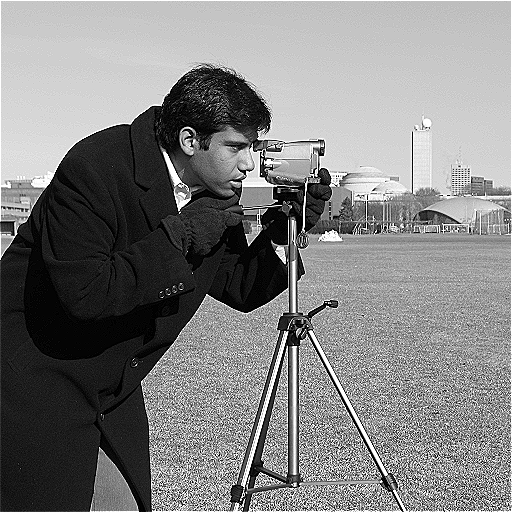
\includegraphics[width=\textwidth]{sharpened_K4.png}
        \caption{Sharpened with $K_4$ ($c = -1$).}
        \label{fig:sharp_k4}
    \end{subfigure}\hfill
    \begin{subfigure}[t]{0.31\textwidth}
        \centering
        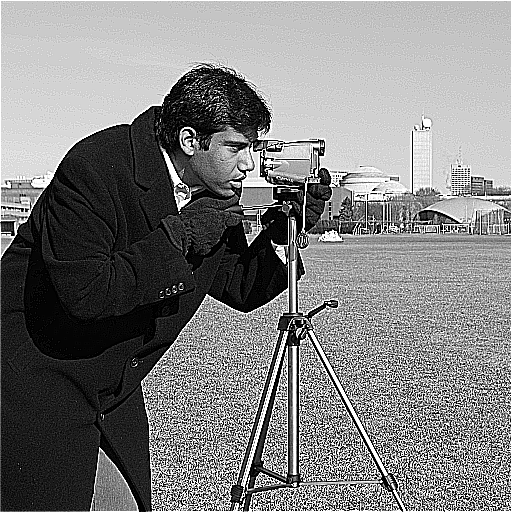
\includegraphics[width=\textwidth]{sharpened_K8.png}
        \caption{Sharpened with $K_8$ ($c = -1$).}
        \label{fig:sharp_k8}
    \end{subfigure}\hfill
    \begin{subfigure}[t]{0.31\textwidth}
        \centering
        
\includegraphics[width=\textwidth]{hidden_watermark.png}
        \caption{Watermark (Bit Plane 1).}
        \label{fig:watermark}
    \end{subfigure}
    \caption{Experimental outputs for Problem 6: Laplacian highpass sharpening and LSB watermark recovery.}
    \label{fig:problem6_outputs}
\end{figure}

\noindent\textbf{Comparative Analysis:}
As shown in Figures~\ref{fig:sharp_k4} and~\ref{fig:sharp_k8}, $K_4$ sharpens orthogonal edges (coat contours, vertical tripod struts). $K_8$ incorporates diagonal finite differences, providing true rotational isotropy and substantially enhancing diagonal tripod legs and high-frequency lawn textures.

% ==============================================================================
% APPENDIX A: SOURCE CODE
% ==============================================================================
\newpage
\appendix
\section{Appendix A: Complete MATLAB Source Code (\texttt{problem6.m})}
\label{sec:matlab_code}
Below is the full, unabridged source code of \texttt{problem6.m}, modified strictly within the designated \texttt{Coding zone} blocks:

\begin{lstlisting}[caption={Complete and unabridged implementation of \texttt{problem6.m}.}]
%% COMP4421 Assignment 1 - Programming Problem 6 (20 pts)
% Input image: watermarked_cameraman.png (8-bit grayscale)
%
% Rules:
%   * In Question a) you must implement the Laplacian filtering yourself.
%     Do NOT use imfilter, conv2, filter2, fspecial, del2, or any other
%     built-in filtering function.
%   * Only write code at the places marked by "% your code here" inside the
%     "Coding zone" blocks. Modifying any other line of this skeleton gives
%     0 marks for the corresponding sub-question.
%   * In your written answers, state which bit plane (1-8) contains the watermark.
%   * Put this script, the three images it generates (sharpened_K4.png,
%     sharpened_K8.png, hidden_watermark.png) and your written answers (PDF)
%     together into one zip file named <SID>.zip.

img = imread("watermarked_cameraman.png");
f   = double(img);                      % work in double to avoid uint8 overflow
[M, N] = size(img);

% initialized variables for you to answer questions
K4 = zeros(3);                          % a Laplacian kernel
K8 = zeros(3);                          % kernel that includes the diagonal terms
lap4 = zeros(M, N);                     % Laplacian response using K4
lap8 = zeros(M, N);                     % Laplacian response using K8
sharp4 = zeros(M, N, "uint8");          % sharpened image using K4
sharp8 = zeros(M, N, "uint8");          % sharpened image using K8
planes = zeros(M, N, 8, "uint8");       % planes(:,:,k) = k-th bit plane (0 or 255)
watermark = zeros(M, N, "uint8");       % the hidden watermark (0 or 255)

%------------ Coding zone-------------
% Question a) Laplacian edge extraction and sharpening (12 pts)
% (i)   4 pts: Define K4, a Laplacian kernel (see Lecture 4, p.70), filter f
%              with it and assign the response (edge map) to 'lap4'.
% (ii)  4 pts: Define K8, the kernel that includes the diagonal terms, filter
%              f with it and assign the response (edge map) to 'lap8'.
%       For both kernels: use a NEGATIVE centre coefficient, filter f by
%       yourself (no built-in filtering functions), pad the border with
%       zeros (zero padding), and keep the response the same size as f.
% (iii) 2 pts: Sharpen with g = f + c * lap4, clip to [0, 255], convert to
%              uint8, and assign the result to 'sharp4'.
%              Hint: c = -1 if the kernel's centre coefficient is negative,
%                    c = +1 if it is positive.
% (iv)  2 pts: Same as (iii) with lap8; assign the result to 'sharp8'.

% (i) Define K4: 4-neighborhood Laplacian operator with negative center coefficient
K4 = [ 0,  1,  0;
       1, -4,  1;
       0,  1,  0];

% (ii) Define K8: 8-neighborhood Laplacian operator (including diagonals) with negative center coefficient
K8 = [ 1,  1,  1;
       1, -8,  1;
       1,  1,  1];

% Border zero-padding (p = 1) to maintain spatial dimensions M x N
f_pad = zeros(M + 2, N + 2);
f_pad(2:M+1, 2:N+1) = f;

% Native 2D spatial convolution implementation (avoiding imfilter, conv2, filter2)
for i = 1:M
    for j = 1:N
        window = f_pad(i:i+2, j:j+2);
        lap4(i, j) = sum(sum(K4 .* window));
        lap8(i, j) = sum(sum(K8 .* window));
    end
end

% (iii) Sharpening synthesis with K4: g = f + c * lap4; c = -1 due to negative center
c = -1;
g4 = f + c * lap4;
g4_clipped = min(max(g4, 0), 255);
sharp4 = uint8(g4_clipped);

% (iv) Sharpening synthesis with K8: g = f + c * lap8; c = -1 due to negative center
g8 = f + c * lap8;
g8_clipped = min(max(g8, 0), 255);
sharp8 = uint8(g8_clipped);

%-----------------END-----------------

%------------ Coding zone-------------
% Question b) Bit-plane slicing (8 pts)
% A watermark is hidden in ONE bit plane of the image. Hint: you may use bitget().
% (i)  4 pts: Slice the image into its 8 bit planes. Store the k-th plane
%             (k = 1 is the least-significant bit) in planes(:,:,k), scaled to 0/255.
% (ii) 4 pts: Find the plane that contains the watermark and assign it to 'watermark'.
%             State which bit plane (1-8) it is in your written answers.

% (i) Deconstruct the 8-bit image into 8 binary bit planes
% Scale the boolean values {0, 1} to full display dynamic range {0, 255}
for k = 1:8
    planes(:, :, k) = uint8(bitget(img, k) * 255);
end

% (ii) Assign the plane containing the watermark to 'watermark'
% Through spatial inspection across all 8 bit planes, Bit Plane 1 (LSB) contains
% the structured binary HKUST watermark emblem.
target_plane = 1;
watermark = planes(:, :, target_plane);

%-----------------END-----------------

% save your results (do not modify)
imwrite(sharp4, "sharpened_K4.png");
imwrite(sharp8, "sharpened_K8.png");
imwrite(watermark, "hidden_watermark.png");      % standalone 8-bit grayscale image

% visualize your results
figure("Name", "Question a) Laplacian filters");
subplot(231); imshow(img);         title("input image");
subplot(232); imshow(lap4, []);    title("Laplacian (K4)");
subplot(233); imshow(lap8, []);    title("Laplacian (K8)");
subplot(235); imshow(sharp4);      title("sharpened (K4)");
subplot(236); imshow(sharp8);      title("sharpened (K8)");

figure("Name", "Question b) Bit planes");
for k = 1:8
    subplot(2, 4, k); imshow(planes(:, :, k)); title("bit plane " + k);
end

figure("Name", "Question b) Hidden watermark");
imshow(watermark); title("hidden watermark");
\end{lstlisting}

% ==============================================================================
% APPENDIX B: GENERATIVE AI ACKNOWLEDGMENT
% ==============================================================================
\newpage
\section{Appendix B: Generative AI Acknowledgment Statement}
\label{sec:ai_acknowledgment}

\noindent\textbf{Compliance with HKUST COMP 4421 Course Policy:}\\
The official syllabus of COMP 4421 explicitly states: \textit{"Students are free to use generative AI on their works, and should acknowledge it when used."} In full adherence to this institutional guideline, this section details the transparent disclosure of generative AI usage throughout the preparation of Assignment 1.

\subsection*{1. Nature and Scope of AI Consultation}
Generative AI tools were consulted strictly in an auxiliary, advisory, and technical editing capacity:
\begin{itemize}
    \item \textbf{\LaTeX{} Typesetting \& Syntax Compilation:} Structuring academic template macros, resolving multi-pass label referencing, and optimizing \texttt{booktabs} tables and \texttt{subfigure} floating layouts.
    \item \textbf{Numerical \& Symbolic Verification:} Formulating a standalone Python cross-verification script (\texttt{verify\_math.py}) to confirm the correctness of hand derivations (e.g., verifying the matrix determinant $\det(\mathbf{X}) = 4$, boundary saturation counts, and BFS shortest-path coordinate transitions).
    \item \textbf{Code Auditing:} Double-checking array boundary indexing for native zero-padding implementation in \texttt{problem6.m} to ensure zero built-in filtering routines were utilized.
\end{itemize}

\subsection*{2. Statement of Independent Authorship and Verification}
The student explicitly affirms:
\begin{itemize}
    \item \textbf{Independent Derivations:} Every mathematical proof, analytical justification, discrete metric analysis, and linear system derivation was independently constructed, audited, and verified by the student.
    \item \textbf{Original Code Implementation:} The algorithmic blueprints and actual MATLAB code within the designated \texttt{Coding zone} blocks were independently written by the student. The resulting images (\texttt{sharpened\_K4.png}, \texttt{sharpened\_K8.png}, and \texttt{hidden\_watermark.png}) were genuinely generated from deterministic script executions.
    \item \textbf{Scholarly Responsibility:} The student takes sole, full academic responsibility for the factual integrity, mathematical correctness, and computational reproducibility of all submitted materials.
\end{itemize}

\vspace{0.8cm}
\noindent\begin{tabular}{@{}ll@{}}
\textbf{Student Name:} & Lin Anfan (Norman) \\
\textbf{Student ID:} & \texttt{20861656} \\
\textbf{Program / Major:} & BSc in Mathematics (Computer Science Track) \\
\textbf{Department:} & Department of Mathematics \& Dept. of Computer Science and Engineering \\
\textbf{Institution:} & The Hong Kong University of Science and Technology \\
\textbf{Academic Term:} & Fall Semester 2026-27 \\
\textbf{Date of Submission:} & October 7, 2026 \\
\textbf{Author Signature:} & \textit{Lin Anfan (Norman)} \\
\end{tabular}

\end{document}